\documentclass[12pt]{article}
\usepackage[utf8]{inputenc}
\usepackage[margin=1in]{geometry}

%Standard Commands
\newcommand{\R}{\mathbb{R}}
\newcommand{\Q}{\mathbb{Q}}
\newcommand{\Z}{\mathbb{Z}}
\newcommand{\N}{\mathbb{N}}
\newcommand{\M}{\mathbb{M}}
\newcommand{\eps}{\varepsilon}
\newcommand{\bs}{\backslash}

%Standard Packages TODO: Figure out what each one does
\usepackage{amssymb}
\usepackage{amsthm}
\usepackage{xcolor}
\usepackage{amsfonts}
\usepackage{graphicx}
\usepackage{float}
\usepackage{amsmath}
\usepackage{version}
\usepackage{caption}
\usepackage{mathtools}
\usepackage{enumerate}
\usepackage{setspace}
\usepackage[parfill]{parskip}

%Standard Theorems
\newtheorem{theorem}{Theorem}
\theoremstyle{definition}
\newtheorem{definition}{Definition}
\newtheorem{example}{Example}
\newtheorem{proposition}{Proposition}
\newtheorem{corollary}{Corollary}
\newtheorem{question}{Question}
\newtheorem{answer}{Answer}

%Doc Info
\title{Volatile Kalman Filter Scaling Law Notes}
\author{Alexander Lanine}
\date{2024-11-25}

\begin{document}
\maketitle

\section*{Introduction}

A central goal for learning theories in psychology and neuroscience is to model how animals and humans learn associations between cues and outcomes. 
Typically, this process is often modeled by updating beliefs based on prediction errors, modulated by a learning rate. 
\textit{Behrens et al.} (2007) proposed that learning rates are dynamically modulated by the \textit{volatility} of the environment: when environmental changes are more frequent, the learning rate should increase, and when changes are less frequent, it should decrease. 
However, the computational model introduced by \textit{Behrens et al.} to describe this relationship is computationally complex and likely not biologically feasible.

To address this, \textit{Piray and Daw} (2020) introduced the \textit{Volatile Kalman Filter} (VKF) as tractable model of learning in volatile environments.
The model has three parameters: the observation noise $\sigma^2$, initial volatility estimate $v_0$, and volatility update parameter $\lambda$. 
At each time step, the posterior mean $m_t$ and variance $w_t$ of the latent state $s_t$ is estimated according to the following algorithm.

\begin{enumerate}
    \item Compute the Kalman Gain: 
    $k_t = (w_{t-1}+v_{t-1})/(w_{t-1}+v_{t-1}+\sigma^2)$

    \item Update the Posterior Mean:
    $m_t = m_{t-1} + k_t(o_t-m_{t-1})$

    \item Update the Posterior Variance: 
    $w_t = (1-k_t)(w_{t-1}+v_{t-1})$

    \item Update Volatility Estimate: 
    $v_t = v_{t-1} + \lambda
        ((m_t-m_{t-1})^2+w_{t-1}+w_t-2w_{t-1,t}-v_{t-1})$
\end{enumerate}
Where $o_t$ is the observation at time $t$ and $w_{t-1,t}$ is the autocovariance $w_{t-1,t} = cov[x_t,x_{t-1}]$ and can be shown to be given by 
$w_{t-1,t} = (1-k_t)w_{t-1}.$

In this project, we investigate how the magnitude of the prediction error $|o_t-m_{t-1}|$ impacts the volatility estimate $v_t$ for both current at future update steps. 
To make this precise, we first let $\mathbf{v} \in \R^T$ denote the volatility estimates given by the VKF for a simulation of $T$ time steps, so that $\mathbf{v}(t) = v_t$. 
Likewise, let $\mathbf{\delta} \in \R^T$ be the same for the magnitude of the prediction error, so $\mathbf{\delta}(t) = |m_{t-1} - o_t|$.
Now, let the rolling average of $\mathbf{\delta}$ at time $t$ be denoted by $\mathbf{\delta}_{\text{avg}}(t)$, which can be computed as
$$
\mathbf{\delta}_{\text{avg}}(t) = \frac{1}{n} \sum_{k=1}^{n_p} \mathbf{\delta}(t-k)
$$
where $n_p \in \mathbb{N}$ is the number of preceding elements included in the average and $\mathbf{\delta}(t-k)$ represents the prediction error at previous time steps. 
We further let $\mathbf{\delta}_{\text{avg}}^n \in \R^{T-n}$ to be the vector containing the rolling averages for time steps $n+1\leq t \leq T$.

We define $n_r \leq T/2$ to be the integer such that maximizes the pearson correlation between $\delta_{\text{avg}}^{n_r}$ and $\mathbf{v}_{n+1:}$. 
Note that we take $n_r \leq T/2$ in all experiments to avoid finding spurious correlations between small vectors.
This condition can likely be considerably relaxed, however. 
Further, we define $n_\rho$ to be the integer that maximizes Spearman's rank correlation coefficient for the same vectors. 

The computational experiments outline below investigate the connection between $n_r$, $n_\rho$, and $\lambda$.
In particular, our main finding will be to demonstrate that 
$$n_r = \frac{c_r}{\lambda}, \: n_\rho = \frac{c_\rho}{\lambda},$$
where $c_r$ and $c_\rho$ depend only on the other parameters in the simulation.

\section*{Experiment One}

In the first experiment, we assume that the latent state dynamics match are those assumed by the derivation of VKF. That is, that the latent state at time $t$ is given by 
$$s_t = s_{t-1}+e_t,$$
where $e_t$ is a noise term drawn from $\mathcal{N}(0,z_t^{-1}).$ 
The precision $z_t$ is updated according to 
$$z_t = Rz_{t-1}\eps_t,$$
where $R \geq 1$ is a constant and $\eps_t$ is a random variable drawn from a beta distribution governed by 
$$p(\eps_t) = \mathcal{B}(\eps_t \vert \eta\nu, (1-\eta)\nu),$$
where $\eta = R^{-1}$ and $\nu = \frac{1}{2(1-\eta)}$.
Observation were generated by the Gaussian distribution
$$p(o_t | s_t)=\mathcal{N}(o_t | s_t, \sigma_o^2),$$
where $\sigma_o^2$ is the observation variance, which is fixed across time. 

First, we ran the simulation of the latent state for $T=500$ time steps with initial latent state and precision $s_0=10$ and $z_0=10$, respectively. 
The observation variance was set at $\sigma_o^2=0.1$, and $(1-\eta) = 0.001$, which controls how the precision $z_t$ is updated over time.
VKF was then run on the observations generated by the simulation with parameters $\lambda = 0.2$, $v_0=1.0$, and $\sigma^2 =0.3$.
Figure \ref{fig:walk_1} depicts the true latent state $s_t$, the predictions of VKF $m_t$, and the observations for each time step. 
Figures \ref{fig:vol_1} and \ref{fig:lr_1} illustrate the volatility estimates and the learning rates (Kalman gain) derived from the simulation, respectively.

\begin{figure}[H]
    \centering
    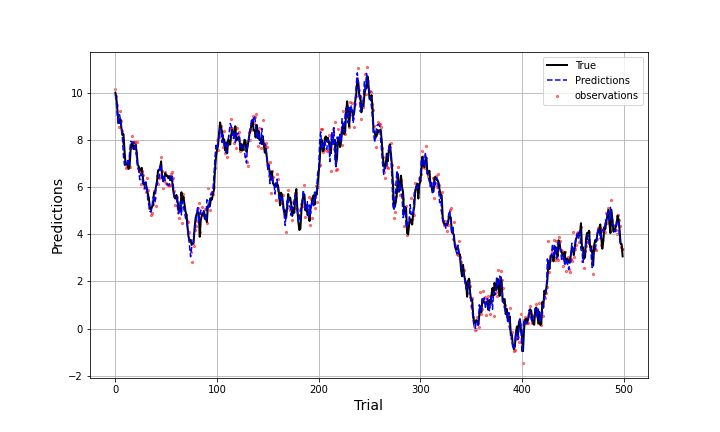
\includegraphics[scale=0.5]{../Figures/exp1_walk.png}
    \caption{Simulation results for $T = 500$ time steps showing the true latent state ($s_t$), the predictions of the Volatile Kalman Filter (VKF; $m_t$), and the observations. The initial latent state and precision were set to $s_0 = 10$ and $z_0 = 10$, respectively, with observation variance $\sigma_o^2 = 0.1$ and precision update parameter $(1-\eta) = 0.001$. VKF was applied to the simulated observations with parameters $\lambda = 0.2$, $v_0 = 1.0$, and $\sigma^2 = 0.3$.
    }
    \label{fig:walk_1}
\end{figure}

\begin{figure}[H]
    \centering
    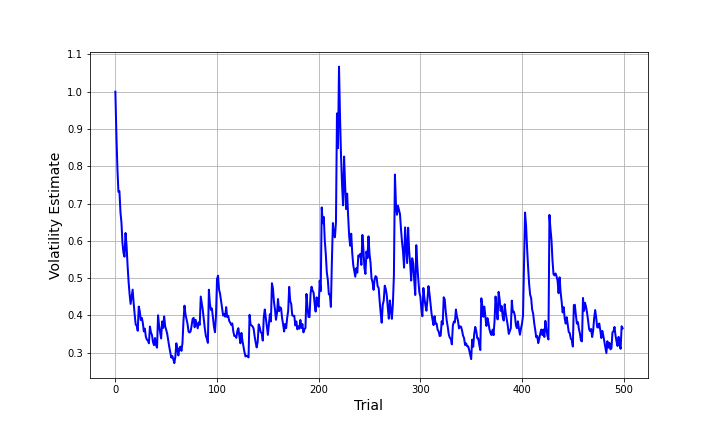
\includegraphics[scale=0.5]{../Figures/exp1_vol.png}
    \caption{Volatility estimates ($v_t$) produced by the Volatile Kalman Filter (VKF) during the simulation of $T = 500$ time steps. The volatility estimate reflects the model's inferred uncertainty about the environment's rate of change, with initial parameters set to $\lambda = 0.2$, $v_0 = 1.0$, and $\sigma^2 = 0.3$.
    }
    \label{fig:vol_1}
\end{figure}

\begin{figure}[H]
    \centering
    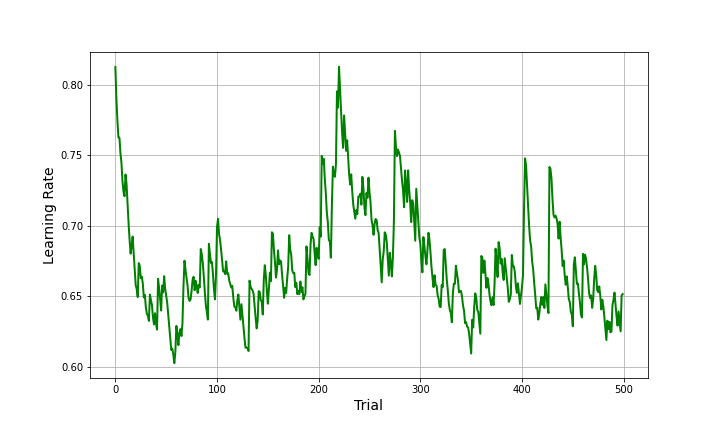
\includegraphics[scale=0.5]{../Figures/exp1_lr.png}
    \caption{Learning rates (Kalman gain, $k_t$) computed by the Volatile Kalman Filter (VKF) for the simulation of $T = 500$ time steps. The Kalman gain adapts dynamically to changes in the environment, influenced by the volatility estimates and observation variance ($\sigma^2 = 0.3$).
    }
    \label{fig:lr_1}

\end{figure}

To further explore the relationship between the magnitude of the prediction error and the volatility estimates, we calculated Pearson and Spearman correlation coefficients between the rolling average of the prediction error $\mathbf{\delta}_{\text{avg}}(t)$ and the volatility estimates $\mathbf{v}(t)$ across varying window sizes $n_p$. The results are shown in Figure \ref{fig:correlation_1}, which depicts the correlation values as a function of the rolling average window size $n_p$.

\begin{figure}[H]
    \centering
    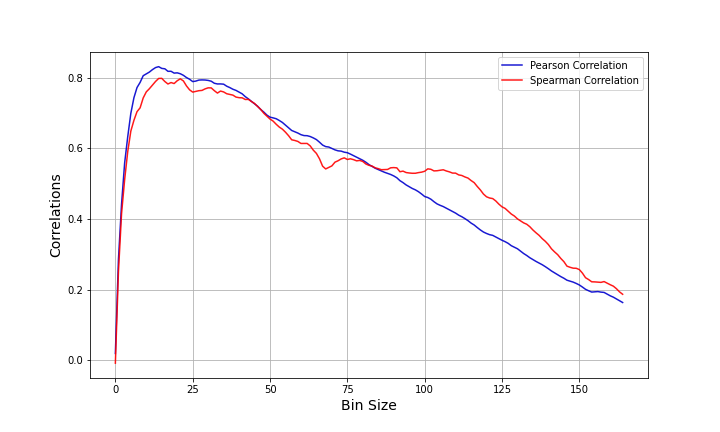
\includegraphics[scale=0.5]{../Figures/correlations1.png}
    \caption{
    }
    \label{fig:correlation_1}
\end{figure}

The plots reveal that the Pearson correlation increases initially with larger window sizes, peaking at $n_r = 14$, indicating the strongest linear relationship for this specific scale. Similarly, the Spearman correlation, which captures monotonic relationships, reaches its maximum at $n_\rho = 15$. 
The trends in both correlation measures decline beyond their respective peaks, indicating that overly large windows dilute the relationship between prediction error and volatility estimates.

To investigate, the relationship between $n_r$, $n_\rho$ and $\lambda$, we repeat the simulation $100$ times, varying $\lambda$ between $10^-2$ and $1$ on a logarithmic scale. 
Figure \ref{fig:exp1_cors.png} shows how illustrates how the optimal rolling average sizes $n_r$ and $n_\rho$ change as a function of $\lambda$


\begin{figure}[H]
    \centering
    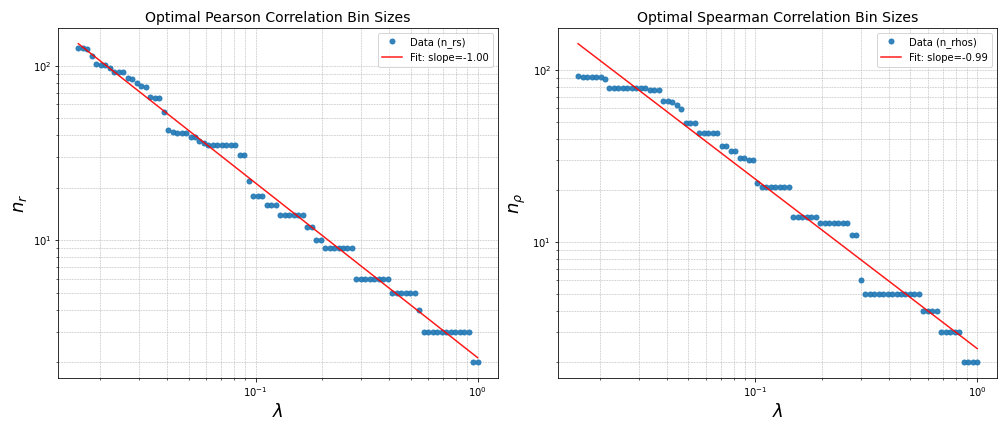
\includegraphics[scale=0.5]{../Figures/regression1.png}
    \caption{Log-log plots of $n_r$ and $n_\rho$ against $\lambda$.}
    \label{fig:exp1_cors.png}
\end{figure}
     
The results show a clear linear relationship on a log-log scale, consistent with the hypothesized inverse proportionality between $n_r$, $n_\rho$ and $\lambda$.
Specifically:
\begin{itemize}
    \item For the Pearson correlation, the slope of the regression line is approximately $-1.00$, with an intercept of $0.33$ and $R^2 = 0.99$. This suggests that the relationship between $n_r$ and $\lambda$ is nearly perfectly described by the equation:
    $$
    n_r \cdot \lambda \approx 2.13.
    $$
    \item For the Spearman correlation, the slope is $-0.99$, with an intercept of $0.38$ and $R^2 = 0.98$. This indicates a similar relationship for $n_\rho$:
    $$
    n_\rho \cdot \lambda \approx 2.41.
    $$
\end{itemize}
\footnote{Due to some numerical issues, I calculated these values using the values from only the last 90 simulations. This can be easily fixed to produce the same result, however (which I may try to do when I have more time\dots).}
\newpage 

\section*{Experiment Two}

Assume that $s_t \sim \mathcal{N}(s_{t-1},\nu)$ for constant process variance $\nu$. Further, assume that 
$$o_t \sim \mathcal{N}(s_t, \sigma_t^2).$$
Throught the trial, observation noise $\sigma_t^2$ switches between two values $\sigma_\ell^2, \sigma_h^2,$ where $\sigma_\ell^2 < \sigma_h^2$.

\textcolor{blue}{Forthcoming.} 

\begin{figure}[H]
    \centering
    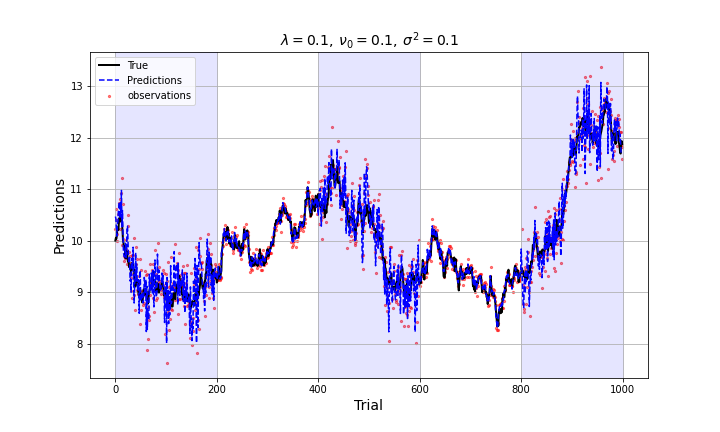
\includegraphics[scale=0.5]{../Figures/exp2_walk.png}
\end{figure}

\begin{figure}[H]
    \centering
    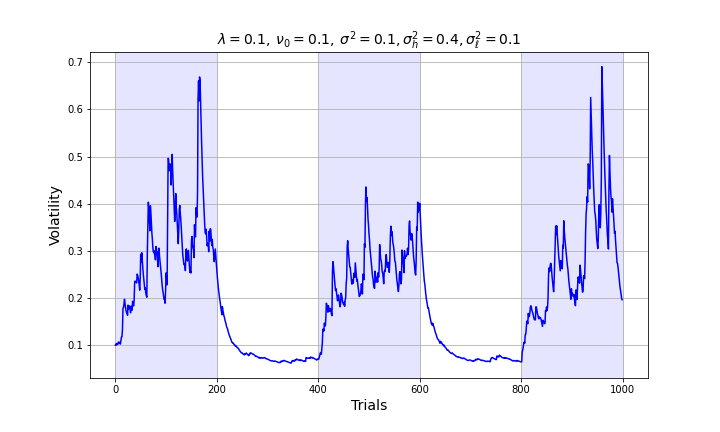
\includegraphics[scale=0.5]{../Figures/exp2_vol.png}
\end{figure}

\begin{figure}[H]
    \centering
    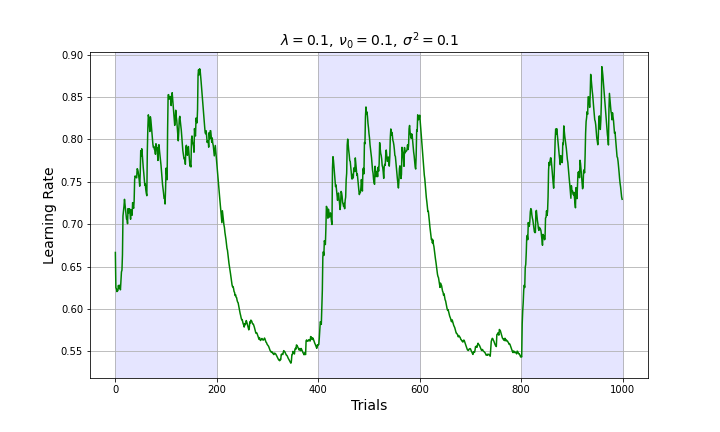
\includegraphics[scale=0.5]{../Figures/exp2_lr.png}
\end{figure}

\begin{figure}[H]
    \centering
    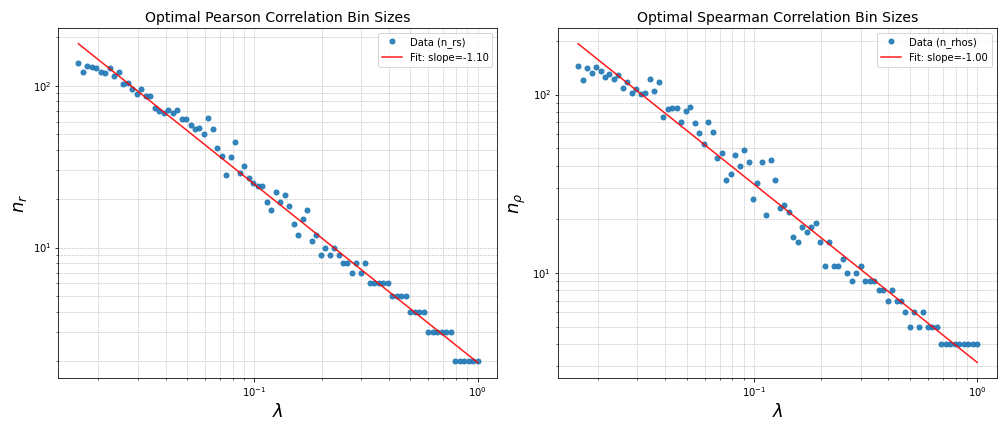
\includegraphics[scale=0.5]{../Figures/regression2.png}
\end{figure}

\end{document}